\section{Introduction}
Motivated by questions in the analysis of practical cryptosystems (block ciphers), we study pseudorandomness properties of random reversible circuits. That is, we study the indistinguishability of truly random permutations on $\{0,1\}^n$ versus permutations computed by small, randomly chosen reversible circuits. 

Our main results concern the extent to which small random reversible circuits compute \emph{approximate $k$-wise independent} permutations. This corresponds to \emph{statistical security} against adversaries that get $k$ input-output pairs from the permutation. 

\subsection{Cryptographic considerations}\label{sec:crypto}
Block ciphers lie at the core of many practical implementations of cryptography. Constructions such as the Advanced Encryption Standard (AES) and Data Encryption Standard (DES) are commonly implemented in hardware on computers as instantiations of pseudorandom permutations, and much is demanded of both their security and efficiency. The need for simple and efficient hardware implementations is often in tension with the hope that these block ciphers are secure against cryptanalysis.

Short of showing unconditional security of a particular block cipher against general polynomial-time adversaries, one might hope to show that random reversible circuits are secure against certain classes of cryptographic attacks. Examples of known attacks against block ciphers include linear cryptanalysis, differential cryptanalysis, higher-order attacks, algebraic attacks, integral cryptanalysis, and more. See, for example, \cite{liu2021t,liu2023layout} and the references therein.

We study a pseudorandomness property that implies security against many of these known classes of attacks:
\begin{definition}
    A distribution $\mathcal{P}$ on permutations of $\{0,1\}^n$ is said to be \emph{$\epsilon$-approximate $k$-wise independent} if for all distinct $x^{(1)}, \dots, x^{(k)} \in \{0,1\}^n$, the distribution of $(\boldsymbol{g}(x^{(1)}), \dots, \boldsymbol{g}(x^{(k)}))$ for $\boldsymbol{g} \sim \mathcal{P}$ has total variation distance at most $\epsilon$ from the uniform distribution on $k$-tuples of distinct strings from~$\{0,1\}^n$.
\end{definition}
By definition, such distributions are statistically secure (up to advantage~$\epsilon$) against an adversary that gets access to any $k$ input-output pairs, chosen non-adaptively. For example, approximate 2-wise independence implies security against linear and differential attacks, and approximate $k$-wise independence for larger $k$ implies security against higher-order differential attacks. Moreover, Maurer and Pietrzak~\cite{maurer2004composition} have shown that this can easily be upgraded to security against \emph{adaptive} queries by composing two draws from the pseudorandom permutation (the second inverted). 

One might be more interested in the security of $\calP$ against any polynomial-time adversary though. Such adversaries can make any polynomial number of queries to the permutation, so to use the security guarantee of approximate $k$-wise independence to infer computational security, one would need to set $k$ to be superpolynomial. A simple argument shows that such permutations require superpolynomial circuit complexity.

However, all known computationally efficient attacks against block ciphers fail as soon as approximate 4-wise independence holds. That is, we know of no approximate 4-wise independent permutation generated as the composition of many local permutations (gates) that is efficiently distinguishable from a completely random permutation of the set of $n$-bit strings. To highlight this fact, it was conjectured in \cite{hoory2005simple} (Section 6) that any $\exp(-n)$-approximate 4-wise independent permutation which is obtained by composing some number of reversible gates forms a pseudorandom permutation. This provides further motivation for the study of approximate $k$-wise independence. 

In addition to providing security guarantees, much focus is put on designing simple and efficient block ciphers. Recall that a random reversible circuit takes as input some $n$-bit string and computes a permutation by letting a sequence of random gates on 3 bits\footnotemark act on the $n$-bit strings.  In this paper we study a natural class of very efficiently implementable circuits, known as brickwork circuits. A brickwork circuit is formed by organizing the bits (also called wires of the circuit) into a low-dimensional lattice and applying layers of gates acting on nearest-neighbors in this lattice at a time. See \Cref{fig:2D brickwork} for an illustration of this architecture. 

\footnotetext{Note that gates that act on three wires are necessary, since the set of gates acting on two wires at a time can generate only $\F_2$-affine permutations of the hypercube. Such permutations do not exhibit nontrivial types of pseudorandomness.} 


The natural efficiency-related question to then ask is how much depth is required for these brickwork circuits to become pseudorandom. In other words, we hope for a class of random reversible circuits that has the following desirable properties:
\begin{itemize}
    \item The gate architecture is fixed and all gates in the circuit act on nearest-neighbor wires in a low-dimensional Euclidean geometry.
    \item The circuits become approximate $k$-wise independent in very low depth.
    \item The circuit yields a straightforward implementation of its inverse.
\end{itemize}
The first item in this list are especially important for implementations in hardware. The second item shows that they can be run for a short amount of time to achieve pseudorandomness, since circuit depth in this setting corresponds to ``wall clock time." Finally, the third item is relevant to efficient decryption. 

In this paper we introduce a construction of a candidate block cipher/pseudorandom permutation from random local circuits that could yield straightforward and efficient implementations in hardware, and our main result shows that this class of random reversible circuits satisfies these desirable properties:
\begin{theorem}\label{thm:2D main}
    For $k \leq 2^{O(\sqrt{n})}$, there is a class of random reversible circuits with a fixed gate architecture on a two-dimensional lattice (\Cref{fig:2D brickwork}) computing permutations that are $2^{-\sqrt{n}k}$-approximate $k$-wise independent at depth $\sqrt{n} \cdot \widetilde{O}(k^3)$.\footnote{Our result holds even when every gate is assumed to be a $\des{2}$ gate. A gate of type $\des{2}$ if (up to ordering the $c$~bits) it is of the form $(x,b) \mapsto (x,b \oplus f(x))$ for some $f : \{0,1\}^{2} \to \{0,1\}$.}
\end{theorem}
\begin{figure}[t]
    \centering
    \includegraphics[width=0.7\linewidth]{2D_brickwork.png}
    \caption{Our two-dimensional brickwork circuit architecture. Each green bar represents a single random 3-bit gate. \Cref{thm:2D main} states that with the stated number of layers of random gates, the permutation becomes $2^{-\sqrt{n}k}$-approximate $k$-wise independent.}
    \label{fig:2D brickwork}
\end{figure}

This result shows that our candidate block cipher becomes secure against a wide class of attacks in very low depth, by setting $k$ to be various small values. If the conjecture from \cite{hoory2005simple} were to hold, then by setting $k=4$, \Cref{thm:2D main} would imply that random brickwork circuits of \emph{sublinear} depth form computationally secure pseudorandom permutations. 

Our construction is a variant of the random reversible circuits introduced by Gowers~\cite{gowers1996almost}. In this initial work, Gowers also analyzed the approximate $k$-wise independence of random reversible circuits. However, we emphasize that this analysis is a departure from the previous literature on approximate $k$-wise independent permutations from random reversible circuits, which has focused on circuits with non-nearest-neighbor gates without fixed architectures. Our main contribution is showing that even with such desirable properties (fixed gate architecture, geometric locality of gates), circuits still exhibit pseudorandomness properties with small size/depth. Note that the AES block cipher also exhibits a similar 2D-lattice-based structure. 

The construction of these structured circuits are partially inspired by the study of \textit{unitary designs} in quantum physics, in particular \cite{brandao2016local,harrow2023approximate}, but the resulting analysis for our case of permutations differs significantly. 

\Cref{thm:2D main} follows from the following two results. First we show that random reversible circuits with fixed \textit{one-dimensional} gate architectures become approximate $k$-wise independent in small depth.

\begin{theorem}\label{thm:1D main}
    A random one-dimensional brickwork circuit (\Cref{fig:nonlocal local brickwork}) of depth $n\cdot\widetilde{O}(k^2)$ computes a permutation that is $2^{-nk}$-approximate $k$-wise independent.
\end{theorem}

Then, we show that instantiating a certain construction of two-dimensional random reversible circuits with the one-dimensional reversible circuits from \Cref{thm:1D main} maintains approximate $k$-wise independence:

\begin{theorem}\label{thm:2D to 1D reduction}
    Suppose there exists a random reversible circuit with a fixed one-dimensional gate architecture that is $2^{-nk}$-approximate $k$-wise independent. Then there exists a class of random reversible circuits with a fixed gate architecture on a two-dimensional lattice computing permutations that are $2^{-\sqrt{n}k}$-approximate $k$-wise independent at depth $\sqrt{n} \cdot \widetilde{O}(k^3)$.
\end{theorem}


\begin{figure}[t]
    \centering 
    \includegraphics[width=\linewidth]{random_circuits.png}
    \caption{The first circuit is an example of a circuit with generic 3-bit gates. The second is an example of a circuit with 1D nearest-neighbor 3-bit gates. The third is an example of a 1D brickwork circuit with five layers.}
    \label{fig:nonlocal local brickwork}
\end{figure}

We prove \Cref{thm:1D main} with a more general quantitative guarantee, which follows immediately from \Cref{thm:one-layer-brickwork}: that a random brickwork circuit of depth $(nk + \log(1/\eps)) \cdot \wt{O}(k)$ computes an $\epsilon$-approximate $k$-wise independent permutation of $\{0,1\}^n$. Note that \Cref{thm:1D main} follows by setting $\epsilon=2^{-nk}$.

We also obtain a generalization of \Cref{thm:2D main} by generalizing \Cref{thm:2D to 1D reduction} to higher-dimensional lattices:
\begin{theorem}\label{thm:genresult}
    For all $3 \leq D \leq O\pbra{\frac{\log n}{\log \log n}}$ a random reversible circuit with a certain $D$-dimensional gate architecture computes permutations that are $2^{-n^{1/D}}$-approximate $k$-wise independent permutations of $\{0,1\}^n$ with depth $\exp(D) \cdot n^{1/D} \cdot \widetilde{O}(k^3)$, given that $k \log k \leq O(n^{1/3})$ and $n$ is large enough.
\end{theorem}

\paragraph{Optimal dependence on $n$.} Note that the dependencies on $n$ in \Cref{thm:2D main}, \Cref{thm:1D main}, and \Cref{thm:genresult} are all tight for the specific gate architectures mentioned in each respective result. This can be seen by a light-cone argument: even approximate 2-wise independence is not possible if there are two wires that cannot influence each other.

\paragraph{On circuit size.} While the parameter we emphasize in our results is depth, it is interesting to note that our high-dimensional circuit achieves a size vs. $\varepsilon$ tradeoff comparable to that of \cite{gretta2024more}. To illustrate this, we set $k=O(1)$. However, we note that our tradeoffs hold for growing $k$ as well; we make this simplification for ease of exposition. 

In our general \Cref{thm:genresult} we show that (given $D = O(\log n/\log\log n)$) a class of random reversible circuits of size $n^{1+1/D} \cdot \exp(D)$ compute $2^{-\Theta(n^{1/D})}$-approximate $k$-wise independent permutations. The tradeoff in \cite{gretta2024more} is that random reversible circuits of size $\widetilde{O}(n^{1+1/D})$ also compute $2^{-\Theta(n^{1/D})}$-approximate $k$-wise independent permutations. 

While we use purely spectral techniques to obtain our results, \cite{gretta2024more} proceeded by proving log-Sobolev inequalities for random walks associated with random reversible circuits. We believe it is interesting that using spectral techniques, we recover similar mixing time results as those obtained from log-Sobolev inequalities.




\subsection{Related Topics in Pseudorandomness}

\paragraph{Unitary designs.} The definition of approximate $k$-wise independence can be framed in terms of approximating a truly random $2^n$-by-$2^n$ permutation matrix by a pseudorandom one up to $k$th moments. If one replaces permutation matrices with general unitary matrices, then one arrives at the definition of an (approximate) unitary $k$-design. An (approximate) unitary $k$-design is a distribution $\mathcal{P}$ on the unitary group that resembles the Haar random measure on the unitary group up to $k$th moments. 

Among various motivations for constructing (approximate) unitary $k$-designs are derandomization of quantum algorithms, modeling of black holes, and the study of topological order. See, for example, \cite{hayden2007black,scott2008optimizing,brandao2016local,dankert2009exact,huang2020predicting}. Often, the goal is to obtain more efficient implementations of unitary designs using small quantum circuits; this goal is similar to the goal of this paper \cite{brandao2016local,hunter2019unitary,haferkamp2021improved,harrow2023approximate,haferkamp2023efficient,chen2024efficient,metger2024simple,chen2024incompressibility,ma2024construct}.

Recently there has been work on reducing the design of approximate unitary $k$-designs to the design of approximate $k$-wise independent permutations. For example, \cite{metger2024simple,chen2024efficient} provides constructions of approximate unitary $k$-designs from approximate $k$-wise independent permutations in a black-box way. These constructions provide further motivation for the study of efficiently generated $k$-wise independent permutations.

\paragraph{Derandomization.} Approximate $k$-wise independent permutation distributions~$\calP$ have many applications outside of cryptography; derandomization, for example~\cite{mohanty2020explicit}. In such applications, another important parameter is the number of truly random ``seed'' bits needed to generate a draw from~$\calP$. By using techniques such as derandomized squaring, one can generally reduce the seed length to $O(nk)$ for any construction; see~\cite{kaplan2009derandomized}. This is true for the results in our paper, and we don't discuss this angle further. We are generally focused on the circuit complexity of our permutations.


\subsection{Techniques and Comparison with Previous Work}
Recall that our main result \Cref{thm:2D main} is about the approximate $k$-wise independence of brickwork circuits of small depth. We arrive at our result via two steps: proving \Cref{thm:1D main} and proving \Cref{thm:2D to 1D reduction}. We first discuss the proof of \Cref{thm:1D main}.

\subsubsection{Spectral Gaps of Structured Random Reversible Circuits}
We prove \Cref{thm:1D main} by lower bounding the spectral gap of the random walk on the set of $k$-tuples of $n$-bit strings associated with a random one-dimensional brickwork circuits. The only prior work on brickwork or nearest-neighbor gates for implementing permutations is work of \cite{feng2024dynamics}, but their results are quantitatively weaker. 

Prior work in this area, which deals with non-nearest-neighbor random gates, proceeded by bounding the spectral gap of the random walk on $k$-tuples induced by a single random $\des{2}$ gate. 

These earlier works bounded the spectral gap using the canonical paths method (\cite{gowers1996almost,hoory2005simple}) or multicommodity flows and the comparison method (\cite{brodsky2008simple}). We depart from these methods and use techniques from the physics literature concerned with the extent to which random \emph{quantum} circuits are \emph{unitary} $k$-designs. Specifically, for \Cref{thm:one-random-nonlocal} we use the  induction-on-$n$ technique developed in \cite{haferkamp2021improved}, and for our main \Cref{thm:one-random-local} we employ the more sophisticated Nachtergaele method~\cite{nachtergaele1996spectral} as in the work of Brand\~{a}o, Harrow, and Horodecki~\cite{brandao2016local}. In fact, it was posed as a question in \cite{brandao2016local} whether their techniques could be extended to construct approximate $k$-wise independent permutations. We answer this question in the affirmative. Our analyses use Fourier and spectral graph theory methods. In both cases, the inductive technique only begins to work for $n \geq \Theta(\log k)$, and for smaller~$n$ we need to base our argument on~\cite{brodsky2008simple}; in the case of nearest-neighbor gates, this requires a further comparison-method based argument.

One can also interpret our result as the construction of a Cayley graph on $\mathfrak{A}_{2^n}$ with spectral gap $\Omega\pbra{1/n2^n}$ and degree $O(n)$. Previous work on this by Kassabov~\cite{kassabov2007symmetric} constructed constant-degree expanders out of Cayley graphs on $\mathfrak{A}_{2^n}$, but it is not clear if this random walk can be implemented by short circuits. Especially for the cryptographic applications of this work, it is important that our random walks have low circuit complexity. 

In the context of non-nearest-neighbor random gates, the best prior result was the following theorem of Brodsky and Hoory for general (non-nearest-neighbor) reversible architecture:
\begin{theorem} \label{thm:BH}
    (\cite{brodsky2008simple}.)
    Consider the permutation on $\{0,1\}^n$ computed by a reversible circuit of $O(n^3 k^2)$ randomly chosen $\des{2}$-gates (meaning in particular that each gate's $3$ fan-in wires are randomly chosen).
    This is $2^{-O(nk)}$-approximate $k$-wise independent.  More generally, such circuits of size $O(n^2 k) \cdot (nk + \log(1/\eps))$ suffices for $\eps$-approximate $k$-wise independence.
\end{theorem}
There is a simple reduction from general gates to nearest-neighbor gates that incurs factor-$\Omega(n)$ size blowup.  Plugging this into \Cref{thm:BH} would yield $2^{-O(nk)}$-approximate $k$-wise independent permutations formed from nearest-neighbor reversible circuits of size $O(n^4 k^2)$. Besides being non-brickwork, this is worse than our \Cref{thm:1D main} by a factor of about~$n^2$.
We should note that Brodsky and Hoory also prove the following:
\begin{theorem} \label{thm:BH2}
    (\cite{brodsky2008simple}.)
    If $k \leq 2^{n/50}$, then \Cref{thm:BH} also holds for random reversible circuits of size $\wt{O}(n^2 k^2 \log(1/\eps))$.
\end{theorem}
\noindent The improved dependence on $n$ in this theorem, namely $\wt{O}(n^2)$, is good, but one should caution that the dependence on $\log(1/\eps)$ is \emph{multiplicative}.  Thus except in the rather weak case when $\eps \gg 2^{-nk}$, this term introduces a factor of at least $nk$ back into the bound, making it worse than \Cref{thm:BH}.

All of the difficulty in our main result \Cref{thm:1D main} comes from analyzing the \emph{spectral gap} of the natural random walk on $k$-tuples of strings arising from picking \emph{one} random nearest-neighbor gate. Note that by spectral gap we actually mean the gap between the top eigenvalue and the next largest eigenvalue, since the chains we work with often are disconnected. We prove:
\begin{theorem} \label{thm:one-random-local}
    Let $P$ be the transition matrix for the random walk on $\{0,1\}^{nk}$ corresponding to one random nearest-neighbor $\des{2}$ gate. Then $P$ has a spectral gap of $1/(n \cdot \wt{O}(k))$.
\end{theorem}
Given this result, \Cref{thm:1D main} follows almost directly by using the \textit{detectability lemma} from Hamiltonian complexity theory~\cite{aharonov2009detectability}, as in analogous results for unitary designs due to~\cite{brandao2016local}. The intermediate step is again proving the one-step spectral gap lower bound.

\begin{theorem} \label{thm:one-layer-brickwork}
    Let $P$ be the transition matrix for the random walk on $\{0,1\}^{nk}$ corresponding to one layer of brickwork gates. Then $P$ has a spectral gap of $\eta \geq 1/\wt{O}(k)$.
\end{theorem}
Note that \Cref{thm:one-layer-brickwork} directly implies \Cref{thm:1D main} by the standard Markov chain mixing time bound using spectral gaps.

We also prove an analogous result to \Cref{thm:one-random-local} in the case of non-nearest-neighbor gates:
\begin{theorem} \label{thm:one-random-nonlocal}
    Let $P$ be the transition matrix for the random walk on $\{0,1\}^{nk}$ corresponding to one random $\des{2}$ gate. Then $P$ has a spectral gap of $\Omega(1/(n k\cdot \log k))$.
\end{theorem}
Although it may look like this result is conceptually dominated by \Cref{thm:one-random-local}, we include it as it has improved $\log k$ factors, and its proof reveals some of the ideas we use in our proof of \Cref{thm:one-random-local}.

\paragraph{Proof ideas.} The idea that underlies the proofs of all of these theorems is to compare the random walks induced by applying random local permutations to $k$-tuples of strings to the random walks induced by completely resampling subsets of bits in every element of a $k$-tuple of strings. The difference between these two operations is essentially the difference between sampling with replacement and sampling without replacement. To illustrate, given a tuple $(x^1,\dots,x^k)$ of strings, let $\bm{F}_S(x^1,\dots,x^k)=(\by^1,\dots,\by^k)$ be a random tuple of strings where for all $a\not\in S$ we have $\by^i_a = x^i_a$, but where each $\by^i_a$ for $a\in S$ is an independent completely random element of $\{\pm1\}$. From this, it is clear that if $S\cup T=[n]$ then $\bm{F}_T\circ\bm{F}_S(x^1,\dots,x^k)$ is a completely random tuple of strings. 

Much of the work in our proofs is showing that in fact, this intuition still approximately holds when $\bm{F}_S$ is replaced with a random local permutation $\bm{\pi}_S$ that only acts on bits in $S$, applied to each element of the tuple, when $S$ is a large enough set. Note that if $(x^1,\dots,x^k)$ is a tuple of strings, then to sample $(\by^1,\dots,\by^k)=(\bm{\pi}_S(x^1),\dots,\bm{\pi}_S(x^k))$ one can equivalently carry out the following process. Consider the substrings $(x^1|_S,\dots,x^k|_S)$. Then, for every $i\in[k]$, resample $\by^i|_S$ from $\{\pm1\}^S$ at random from the remaining available strings (noting that the $\by^i|_S$ must be distinct for distinct $x^i|_S$. If $S$ is a large enough set, and the strings $x^1|_S,\dots,x^k|_S$ were all distinct, then this process strongly resembles the process of drawing each $\by^i|_S$ independently. In this sense, for such tuples $(x^1,\dots,x^k)$, we have the following resemblance in distributions:
\begin{align}\label{eq:approximation of permutations}
    (\bm{\pi}_S(x^1),\dots,\bm{\pi}_S(x^k)) \approx \bm{F}_S(x^1,\dots,x^k).
\end{align}
On the other hand, if the $x^1|_S,\dots,x^k|_S$ were not distinct, then we use a simple argument based on escape probabilities to show that such tuples also exhibit good expansion.

Equipped with this comparison, we are able to prove statements of the form 
\begin{align*}
    (\bm{\pi}_T\bm{\pi}_S(x^1),\dots,\bm{\pi}_T\bm{\pi}_S(x^k)) \approx \bm{F}_T\bm{F}_S(x^1,\dots,x^k)
\end{align*}
when $S$ and $T$ satisfy certain properties, such as having sufficiently large overlap. When $S\cup T=[n]$ it turns out that the distribution on the right-hand side is equal to a completely random $k$-tuple of $n$-bit strings. Via a lemma of Nachtergaele~\cite{nachtergaele1996spectral} from quantum physics, a linear-algebraic formalization of this approximation results in a large spectral gap for the spectral gaps associated with geometrically-local random reversible circuits.




\subsubsection{Two-Dimensional Construction}
To obtain the reduction \Cref{thm:2D to 1D reduction} we use a technique inspired by \cite{harrow2023approximate}, which obtained a similar reduction in setting of constructing unitary $k$-designs using random quantum circuits. However, there are some complications that arise when working with permutations rather than general unitaries, so our approach departs significantly from that of \cite{harrow2023approximate}.

Our construction, however, is essentially identical to that of \cite{harrow2023approximate}. Let $\mcB$ be a distribution on circuits computing an approximately $k$-wise independent permutation of $\{0,1\}^{\sqrt{n}}$. Let $X \in \{\pm1\}^{\sqrt{n}\times \sqrt{n}}$ be input to our circuit in the form of a two-dimensional lattice, a grid. 
\begin{enumerate}
    \item For each row in $X$, we sample independent circuits from $\mcB$ and apply in parallel.
    \item For each column in $X$, we sample independent circuits from $\mcB$ and apply in parallel.
    \item We repeat steps and 1 and 2 a total of $O(k\log k)$ times, and finally step 1 exactly once more.
\end{enumerate}

What we get as a result is a circuit of $2t+1$ ``layers'', with each layer consisting of $\sqrt{n}$ parallel circuits from the family $\mcB$ all in one of two directions in our lattice. If the circuits in $\mcB$ have depth $d$ then the depth of our circuit is $O(k\log k) \cdot d$.

\begin{figure}[h]
    \centering
    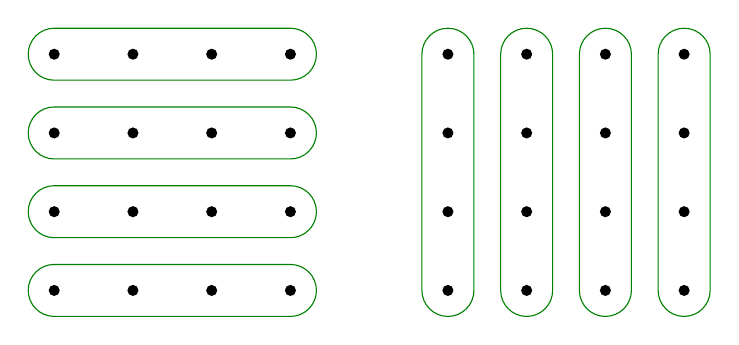
\begin{tikzpicture}
        \def \width {0.33};
        % Row Circuits
        \foreach \y in {0, 1, 2, 3} {
            \filldraw[fill=white, draw=green!50!black] (0,\y-\width) -- (3, \y-\width) arc[start angle=-90, end angle=90, radius=\width] -- (0, \y+\width) arc[start angle=90, end angle=270, radius=\width] -- cycle;
        }
    
        % Grid 1
        \foreach \x in {0, 1, 2, 3} {
            \foreach \y in {0, 1, 2, 3} {
                \fill (\x,\y) circle (2pt);
            }
        }

         % Column Circuits
        \foreach \x in {5, 6, 7, 8} {
            \filldraw[fill=white, draw=green!50!black] (\x-\width, 0) -- (\x-\width, 3) arc[start angle=180, end angle=0, radius=\width] -- (\x+\width, 0) arc[start angle=0, end angle=-180, radius=\width] -- cycle;
        }
    
        % Grid 2
        \foreach \x in {5, 6, 7, 8} {
            \foreach \y in {0, 1, 2, 3} {
                \fill (\x,\y) circle (2pt);
            }
        }
    \end{tikzpicture}
    \vspace{10px}
    \caption{Step 1 applies parallel circuits from $\mcB$ to the rows, while Step 2 applies to the columns. Our circuit alternates between layers of the two.}
    \label{fig:gridcircuit}
\end{figure}
We show that the circuit construction above computes permutations that are $\varepsilon$-approximate $k$-wise independent.

\paragraph{Proof ideas.} As in the 1D case, we reduce analyzing $k$-wise independence of our random reversible circuits to the analyzing the natural induced Markov chain on $\{0,1\}^{nk}$. The induced circuit distribution being approximately uniform then corresponds to mixing in the Markov chain which can be accomplished via establishing a spectral gap or a log-Sobolev inequality.

Our proof does not rely on log-Sobolev inequalities, but rather proceeds entirely through spectral arguments about the random walk operators. However, for sublinear-in-$n$ mixing time (corresponding to circuit depth), it does not suffice to prove a simple spectral gap for our random walk. The reason for this is that naively bounding the mixing time using the spectral gap immediately results in a mixing time at least $\Theta(\log(2^{nk}))=\Theta(nk)$. Thus, we need to proceed more carefully by expressing the total variation distance (which is an $\ell_1$ distance) of the distributions induced by running the Markov chain for some number of steps more directly in terms of the spectral properties of the transition matrices. 

In particular, we derive approximations that resemble those of the type in \Cref{eq:approximation of permutations}, but now the quality of the approximation depends on how many substring collisions the tuple $(x^1,\dots,x^k)$ has. To formalize this quantitatively, we assign each tuple $(x^1,\dots,x^k)$ to a certain group of tuples based on the collision pattern it experiences. By bounding the contribution to the total variation distance of each group of tuples and analyzing the transition probabilities between these groups, we can directly analyze the mixing time without directly exhibiting a functional inequality for the corresponding Markov chain.



\subsection{Comparison with Subsequent Work}\label{sec:subsequent work}
Since the release of the first version of this work, there have been a number of subsequent works on approximate $k$-wise independent permutations and unitary $k$-designs. Of these, perhaps the most relevant to this work are the recent results in \cite{gretta2024more} and \cite{chen2024incompressibility}:
\begin{theorem}[\cite{gretta2024more}, Theorem 2]\label{thm:gretta}
    For any $n$ and $k\leq 2^{n/50}$, a random reversible circuit with $\wt{O}(nk\cdot \log(1/\varepsilon))$ $\des{2}$ gates computes an $\epsilon$-approximate $k$-wise independent permutation.
\end{theorem}


\begin{theorem}[\cite{chen2024incompressibility}, Corollary 1.3]\label{thm:chen}
    For any $n\geq4$ and $k\leq \Theta(2^{n/6.1})$, a random reversible circuit with $\wt{O}(n(nk+\log(1/\varepsilon)))$ $\des{2}$ gates computes an $\epsilon$-approximate $k$-wise independent permutation.
\end{theorem}

It is worth noting the ways in which our results, \Cref{thm:gretta}, and \Cref{thm:chen} supersede each other and are incomparable. We first note that the size bound of $\wt{O}(nk(nk+\log(1/\epsilon))$ implied by \Cref{thm:one-random-nonlocal} is immediately superseded by both \Cref{thm:gretta} and \Cref{thm:chen}.\footnote{In this discussion we ignore factors logarithmic in $n$ and $k$.}

However, the main results of this paper on random reversible circuits with nearest-neighbor gates (\Cref{thm:one-random-local}) and random brickwork circuits (\Cref{thm:1D main}) are still the state-of-the-art. Subsequent works \cite{gretta2024more} and \cite{chen2024incompressibility} say nothing more about reversible circuits with such structured gates than what can be deduced by an application of the comparison method as in \Cref{lem:initial spectral gap local random gates large k}. Such an application immediately incurs a $\mathrm{poly}(n)$ blow-up in the size of the circuits. 

\cite{chen2024incompressibility} claims that it is likely that their techniques can be adapted to show a $\wt{O}(1/n)$ bound on the spectral gap of the random walk induced by one layer of a random brickwork circuit. On the other hand, our spectral gap is $\wt{O}(1/k)$. Thus, if such a result were to be proved, it would be an improvement only if $k$ exceeds $n$. We emphasize that for many purposes one might be interested in the case where $k$ is a constant and $n$ grows. See, for example, the discussion in \Cref{sec:crypto} on a conjecture of \cite{hoory2005simple}.



\subsection{Organization}
The proof of \Cref{thm:1D main} spans \Cref{sec:spectral gaps} and \Cref{sec:nachtergaele hypothesis}. In between, we give a brief overview of our techniques in \Cref{sec:overview} and then prove the separate but related \Cref{thm:one-random-nonlocal} in \Cref{sec:small k}.

The proof of \Cref{thm:2D to 1D reduction} is contained in \Cref{sec:proof of 2D to 1D reduction} and \Cref{sec:spectralproof}, and we prove the more general result about higher-dimensional lattices in \Cref{sec:generallattices}.

